\documentclass[12pt,titlepage]{article}
\usepackage[margin=1.25in]{geometry}
\usepackage{graphicx,amsmath,blindtext}

%% Variables definition
\newcommand{\vSubject}{Basic Programming Practicum}
\newcommand{\vSubtitle}{Jobsheet 5 Assignment}
\newcommand{\vName}{Dicha Zelianivan Arkana}
\newcommand{\vNIM}{2241720002}
\newcommand{\vClass}{1i}
\newcommand{\vDepartment}{Information Technology}
\newcommand{\vStudyProgram}{D4 Informatics Engineering}

%% [START] Tikz related stuff
\usepackage{tikz}
\usetikzlibrary{svg.path,calc,shapes.geometric,shapes.misc}
\tikzstyle{terminator} = [rectangle, draw, text centered, rounded corners = 1em, minimum height=2em]
\tikzstyle{preparation} = [chamfered rectangle, chamfered rectangle sep=0.75em, draw, text centered, minimum height = 2em]
\tikzstyle{process} = [rectangle, draw, text centered, minimum height=2em]
\tikzstyle{decision} = [diamond, aspect=2, draw, text centered, minimum height=2em]
\tikzstyle{data}=[trapezium, draw, text centered, trapezium left angle=60, trapezium right angle=120, minimum height=2em]
\tikzstyle{connector} = [line width=0.25mm,->]
%% [END] Tikz related stuff

%% [START] Fancy header related stuff
\usepackage{fancyhdr}
\pagestyle{fancy}
\setlength{\headheight}{15pt} % compensate fancyhdr style
\fancyhead{}
\fancyfoot{}
\fancyfoot[L]{\thepage}
\fancyfoot[R]{\textit{\vSubject - \vSubtitle}}
\renewcommand{\footrulewidth}{0.4pt}% default is 0pt, overline for footer
%% [END] Fancy header related stuff

%% [START] Custom tabular command related stuff
\usepackage{tabularx}
\newcommand{\details}[2]{
    #1 & #2  \\
}
%% [END] Custom tabular command related stuff

%% [START] Figure related stuff
\newcommand{\image}[3][1]{
    \begin{figure}[h]
        \centering
        \includegraphics[#1]{#2}
        \caption{#3}
        \label{#3}
    \end{figure}
}
%% [END] Figure related stuff

\begin{document}
\begin{titlepage}
    \centering
    \vfill
    {\bfseries\LARGE
        \vSubject\\
        \vskip0.25cm
        \vSubtitle
    }
    \vfill
    
\includegraphics[width=6cm]{images/polinema-logo.png}
    \vfill
    {
        \textbf{Name}\\
        \vName\\
        \vskip0.5cm
        \textbf{NIM}\\
        \vNIM\\
        \vskip0.5cm
        \textbf{Class}\\
        \vClass\\
        \vskip0.5cm
        \textbf{Department}\\
        \vDepartment\\
        \vskip0.5cm
        \textbf{Study Program}\\
        \vStudyProgram
    }
\end{titlepage}

\section{Assignment}
\begin{enumerate}
    \item {
        Using three values that represent the lengths of the three sides of a triangle, determine
        whether the triangle is \textbf{equilateral} (all three sides are equal), \textbf{isosceles} (both sides are
        equal), or \textbf{arbitrary} (no sides are equal)!

        \begin{figure}[h]
            \centering
            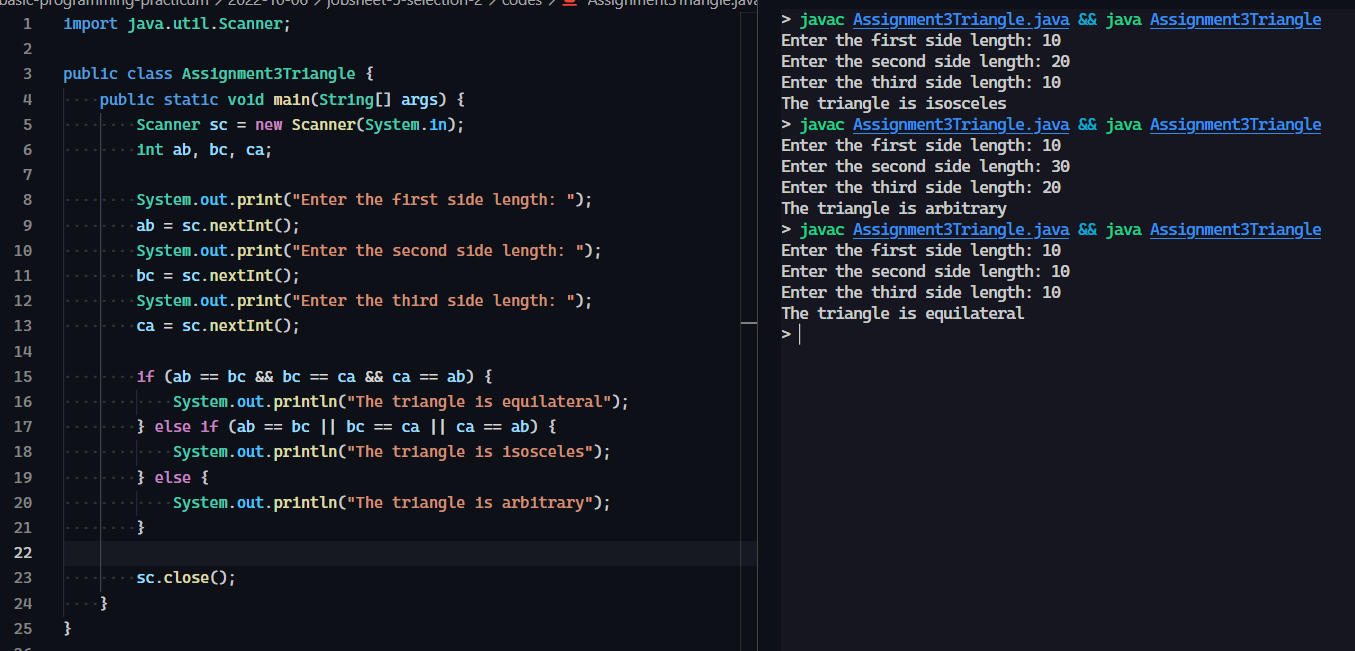
\includegraphics[width=\textwidth]{images/assignment3-triangle.png}
            \caption{Code and output to find triangle sides}
        \end{figure}
    }
    \pagebreak
    \item {
        A restaurant asks you to create a program for taking orders from the internet. The
        program you created asks the user to enter a food name and price. After that, the user is
        offered to use express delivery. If the user refuses, the delivery type used is regular
        delivery. Regular delivery costs for food less than IDR 100,000 are IDR 20,000, while for
        food prices equal to or more than IDR 100,000 the delivery cost is IDR 30,000. For express
        delivery, add an additional fee of IDR 25,000 from the standard regular shipping cost.
        Show a receipt containing the name of the food purchased + price, shipping costs and the
        total to be paid!

        \begin{figure}[h]
            \centering
            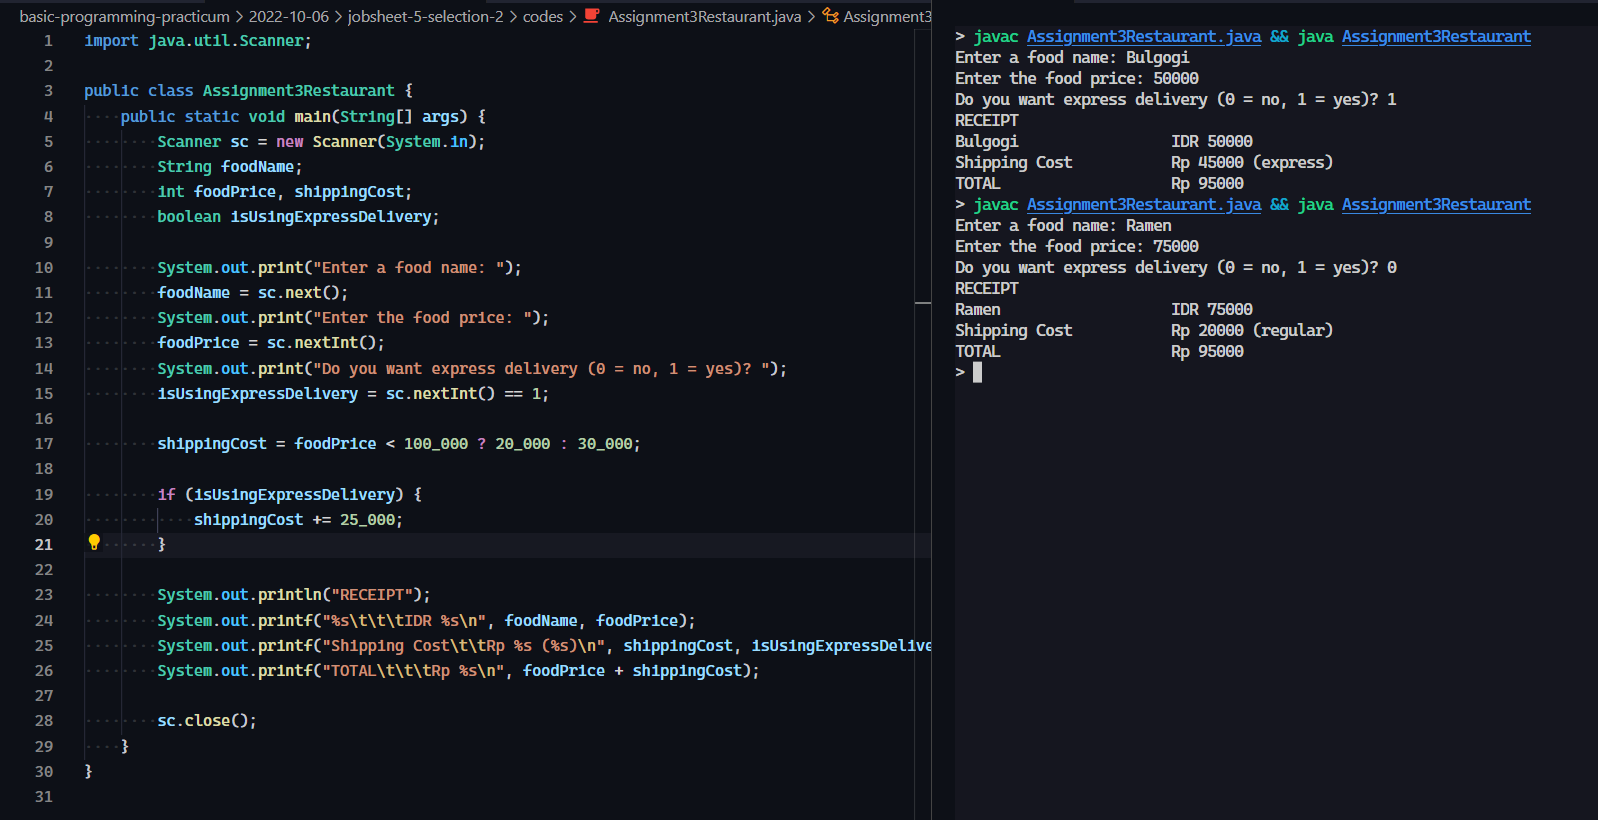
\includegraphics[width=\textwidth]{images/assignment3-restaurant.png}
            \caption{Code and output to calculate total price for a restaurant}
        \end{figure}
    }
\end{enumerate}

\end{document}

